%%%%%%%%%%%%%%%%%%%%%%%%%%%%%%%%%%%%%%%%%%%%%%%%%%%%%%%%%%%%%%%%%%%%%%
%     File: ExtendedAbstract_intro.tex                               %
%     Tex Master: ExtendedAbstract.tex                               %
%%%%%%%%%%%%%%%%%%%%%%%%%%%%%%%%%%%%%%%%%%%%%%%%%%%%%%%%%%%%%%%%%%%%%%

\section{Introduction}
\label{sec:intro}

Referring expression segmentation represents a fundamental advancement in computer vision, enabling models to identify and segment objects based on natural language descriptions rather than predefined category labels. This capability bridges the gap between human language understanding and visual perception, allowing for more intuitive and flexible interaction with computer vision systems. While significant progress has been achieved in natural scene referring expression segmentation, aerial imagery remains largely unexplored despite its critical importance in applications ranging from urban planning and environmental monitoring to autonomous navigation and disaster response.

Aerial imagery presents distinct challenges that differentiate it fundamentally from natural scene photography. Objects in aerial images exhibit extreme density variations, with single images potentially containing hundreds of vehicles, buildings, or infrastructure elements. The top-down perspective creates unique spatial relationship patterns not present in ground-level photography, where traditional concepts like "above" and "below" take on different meanings within the context of geographic positioning. Additionally, aerial images capture vast scale variations, from individual vehicles measuring mere pixels to large building complexes spanning significant portions of the image frame.

\begin{figure}[H]
\centering
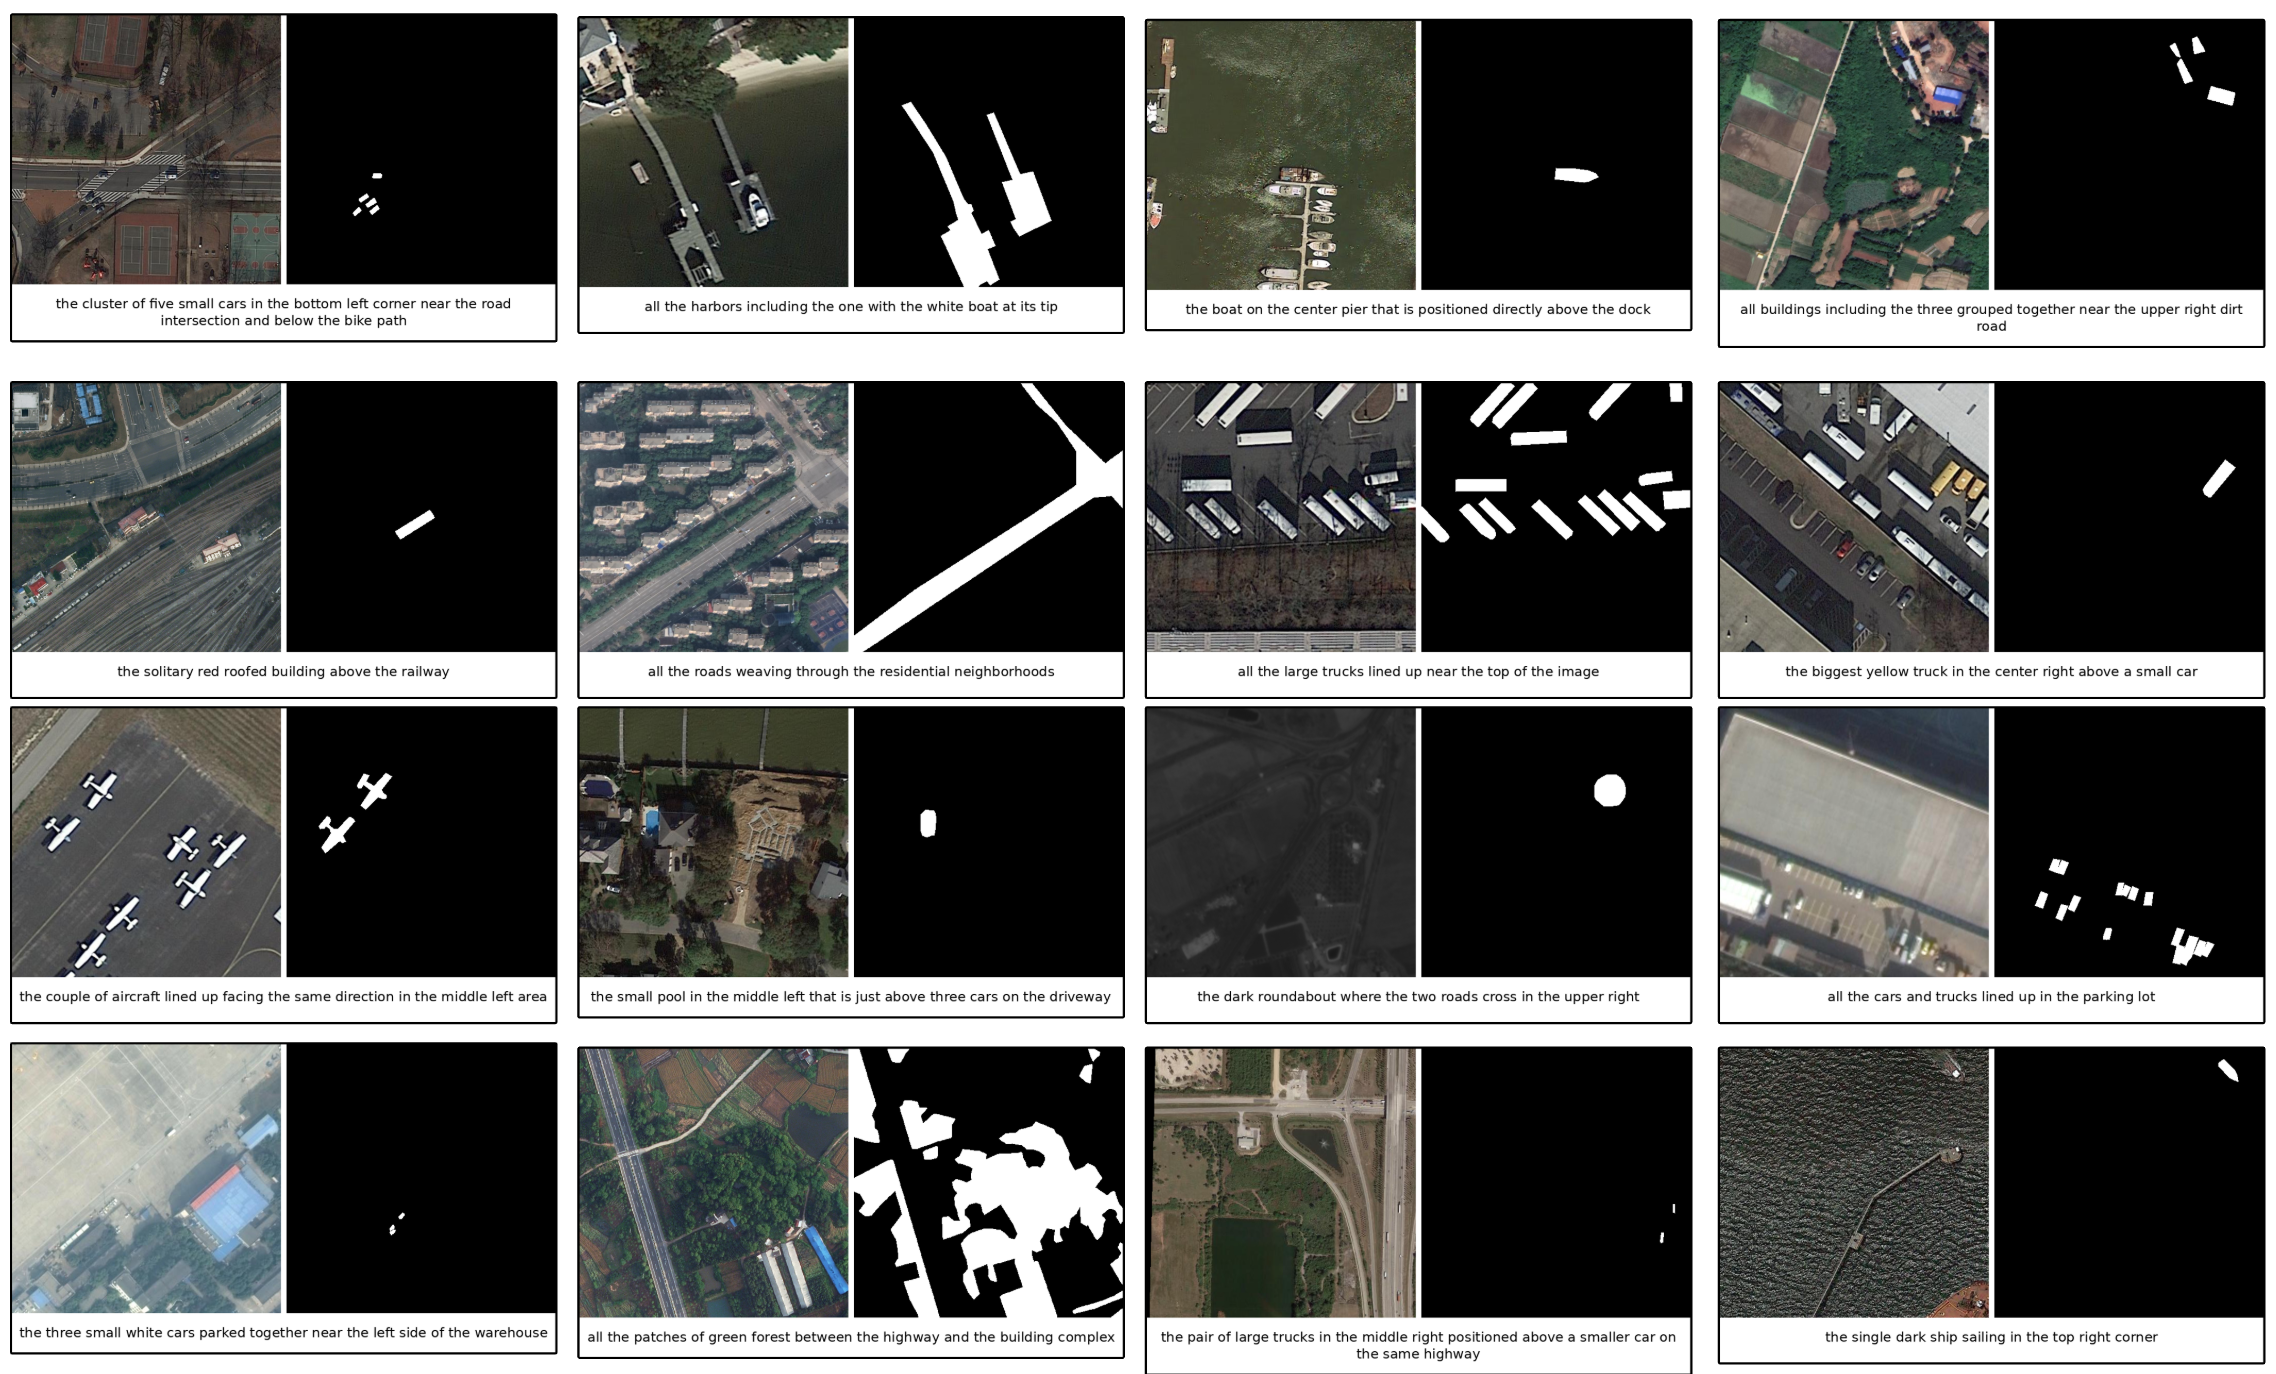
\includegraphics[width=\columnwidth]{./images/dataset.png}
\caption{Representative examples from Aerial-D dataset showing diverse referring expressions with corresponding aerial images and ground truth masks.}
\label{fig:dataset_examples}
\end{figure}

Existing referring expression datasets, including RefCOCO, RefCOCO+, and RefCOCOg, focus exclusively on natural scenes with ground-level photography. These datasets typically contain objects with familiar human-centric spatial relationships and conventional viewing angles. The linguistic patterns and spatial reasoning required for aerial imagery fundamentally differ from these established benchmarks, necessitating specialized dataset construction approaches that can capture the unique characteristics of overhead perspectives.

Current aerial image datasets, such as iSAID and LoveDA, provide excellent resources for traditional object detection and semantic segmentation tasks but lack the natural language component essential for referring expression applications. This limitation prevents the development and evaluation of aerial-specific referring segmentation models, creating a significant gap in the computer vision research landscape. The absence of large-scale aerial referring expression datasets has hindered progress in developing models capable of understanding complex spatial relationships and object descriptions within aerial contexts.

To address these limitations, we present Aerial-D, the first comprehensive referring expression segmentation dataset specifically designed for aerial imagery. Our dataset construction approach combines systematic rule-based expression generation with large language model enhancement to create diverse, natural, and contextually rich referring expressions. The resulting dataset contains over 1.5 million expressions across 37,288 aerial image patches, representing the largest collection of aerial referring expressions available to the research community.

Our key contributions include: (1) the introduction of Aerial-D, the first large-scale aerial referring expression segmentation dataset with over 1.5 million expressions, (2) a fully automatic dataset construction pipeline that leverages rule-based generation and LLM enhancement techniques, (3) comprehensive benchmarking results demonstrating the unique challenges of aerial referring expression segmentation, and (4) cross-dataset evaluation showing good generalization performance of models trained on our dataset.

